\documentclass{article}


\usepackage[preprint]{utils_packages/neurips_2023}



\usepackage[utf8]{inputenc} % allow utf-8 input
\usepackage[T1]{fontenc}    % use 8-bit T1 fonts
\usepackage{hyperref}       % hyperlinks
\usepackage{url}            % simple URL typesetting
\usepackage{booktabs}       % professional-quality tables
\usepackage{amsfonts}       % blackboard math symbols
\usepackage{nicefrac}       % compact symbols for 1/2, etc.
\usepackage{microtype}      % microtypography
\usepackage{xcolor}         % colorsp
\usepackage{float}
\usepackage{listings}
\usepackage{graphicx}
\usepackage{multirow}

\urlstyle{same}
\hypersetup{
  hidelinks,
  pdfcreator={LaTeX via pandoc}}

\author{}
\date{}


\newcommand{\adaev}{\textsc{AdaEvolve}}

\newcommand{\Eric}[1]{{\color{mint}[Eric: #1]}}
\definecolor{mint}{RGB}{62, 180, 137}
% [Custom packages] from here down 
% [Custom packages] from here down 
\usepackage{float}
\usepackage{todonotes}
\usepackage{amsmath}
\usepackage{algorithm}
\usepackage{algpseudocode}
\usepackage{enumitem}
\usepackage{caption}
\usepackage{subcaption}
% \usepackage{biblatex}
% \addbibresource{refs.bib}

\newcommand{\x}{\boldsymbol{x}}
% \newcommand{\y}{\boldsymbol{y}}
\newcommand{\X}{\boldsymbol{X}}
\newcommand{\w}{\boldsymbol{w}}
\newcommand{\sign}{\text{sign}}
\newcommand{\ub}{\boldsymbol{u}}
\newcommand{\z}{\boldsymbol{z}}
\newcommand{\vb}{\boldsymbol{v}}

\newcommand{\numberset}{\mathbb}
\newcommand{\N}{\numberset{N}}
\newcommand{\Z}{\numberset{Z}}
\newcommand{\Q}{\numberset{Q}}
\newcommand{\R}{\numberset{R}}
\newcommand{\C}{\numberset{C}}
\newcommand{\E}{\numberset{E}}
\newcommand{\Prob}{\numberset{P}} 

\usepackage{mathtools}
\DeclarePairedDelimiter\ceil{\lceil}{\rceil}
\DeclarePairedDelimiter\floor{\lfloor}{\rfloor}
\newcommand{\norm}[1]{\left\lVert#1\right\rVert}

\usepackage{nomencl}
\def\bmat#1{\left[\begin{array}{#1}}
\def\emat{\end{array}\right]}
\def\bv {\bmat{c} }
\def\ev {\emat}

\newcommand {\bsis} {\left\{ \begin{array} }
\newcommand {\esis} {\end{array}\right.}

\def\Sum#1#2{\sum\limits_{#1}^{#2}}
\def\set#1#2{\{ \; #1 \;:\;#2\;\}} % creates a set: { #1 : #2 }



\newcommand{\y}{\hat{y}}

\newcommand{\tauB}{\boldsymbol{\tau}}
\newcommand{\xiB}{\boldsymbol{\xi}}
\newcommand{\thetaB}{\boldsymbol{\theta}}
\newcommand{\thB}{{\boldsymbol{\theta}}}
\newcommand{\alB}{{\boldsymbol{\alpha}}}
\newcommand{\betB}{{\boldsymbol{\beta}}}
\newcommand{\yB}{{\boldsymbol{y}}}


\setcounter{MaxMatrixCols}{20}
\newtheorem{remark}{Remark}[section]


% [Custom packages] from here up 

\usepackage{amsmath}

\usepackage{comment}

% [Custom packages] from here up 

\newcommand{\promptdiagram}{%
\vspace{4pt}%
  \noindent\textbf{\small Different parent program (hit rate 0\%):}
  \par\vspace{3pt}%
  \noindent
  \colorbox{berkeleyblue!15}{%
    \begin{minipage}[c][3.0em]{\dimexpr0.18\linewidth-2\fboxsep\relax}%
      \centering\scriptsize system\\[-1pt]
      \tiny 222 tok\\[-1pt]
      \tiny pfx 100\%, mat 100\%
    \end{minipage}}%
  \makebox[0pt][c]{\Large$|$}%
  \colorbox{red!18}{%
    \begin{minipage}[c][3.0em]{\dimexpr0.18\linewidth-2\fboxsep\relax}%
      \centering\scriptsize current program\\[-1pt]
      \tiny 1{,}500 tok\\[-1pt]
      \tiny pfx 10.0\%, mat 50.0\%
    \end{minipage}}%
  \makebox[0pt][c]{\Large$|$}%
  \colorbox{cyan!20}{%
    \begin{minipage}[c][3.0em]{\dimexpr0.64\linewidth-2\fboxsep\relax}%
      \centering\scriptsize other context programs\\[-1pt]
      \tiny 8{,}000 tok\\[-1pt]
      \tiny pfx 1.0\%, mat 70.0\%
    \end{minipage}}%
    
  \vspace{4pt}%

  % ================= SAME PARENT =================
  \noindent\textbf{\small Same parent program (hit rate 34\%):}
  \par\vspace{3pt}%
  \noindent
  \colorbox{berkeleyblue!15}{%
    \begin{minipage}[c][3.0em]{\dimexpr0.18\linewidth-2\fboxsep\relax}%
      \centering\scriptsize system\\[-1pt]
      \tiny 222 tok\\[-1pt]
      \tiny pfx 100\%, mat 100\%
    \end{minipage}}%
  \makebox[0pt][c]{\Large$|$}%
  \colorbox{berkeleygold!40}{%
    \begin{minipage}[c][3.0em]{\dimexpr0.18\linewidth-2\fboxsep\relax}%
      \centering\scriptsize current program\\[-1pt]
      \tiny 1{,}500 tok tok\\[-1pt]
      \tiny pfx 100\%, mat 100\%
    \end{minipage}}%
  \makebox[0pt][c]{\Large$|$}%
  \colorbox{cyan!20}{%
    \begin{minipage}[c][3.0em]{\dimexpr0.64\linewidth-2\fboxsep\relax}%
      \centering\scriptsize other context programs\\[-1pt]
      \tiny 8{,}000 tok\\[-1pt]
      \tiny pfx 29.0\%, mat 75.8\%
    \end{minipage}}%

  % =============== DIFFERENT PARENT ===============


}



\title{EvoScale: Parallel, Cache-Aware Evolutionary Algorithms}

% The \author macro works with any number of authors. There are two commands
% used to separate the names and addresses of multiple authors: \And and \AND.
%
% Using \And between authors leaves it to LaTeX to determine where to break the
% lines. Using \AND forces a line break at that point. So, if LaTeX puts 3 of 4
% authors names on the first line, and the last on the second line, try using
% \AND instead of \And before the third author name.
\author{
Group 7 \\ Matteo Guarrera \quad Elizabeth Polito \quad Harper Lyu \\ Mert Cemri \quad Sultan Daniels \quad Eric Xu
}

\begin{document}
\maketitle
% \vspace{-5cm}
\author{}
% 
\vspace{-0.5cm}

\vspace{-0.3cm}






\section{Introduction}

Evolutionary program search has emerged as a powerful framework for
LLM-guided discovery: a population of candidate programs is iteratively
sampled, mutated by an LLM, and evaluated against a fixed objective,
with the best solutions propagating forward across generations. Recent
open-source systems such as SkyDiscover's \adaev{}~\cite{cemri2026skydiscover},
OpenEvolve~\cite{rudes2025openevolve}, and GigaEvo~\cite{khrulkov2025gigaevo}
have made this paradigm accessible, but they were designed with
closed-source, remotely-hosted LLMs in mind. In that setting, the
inference cost is a pricing concern rather than a systems one; the user
pays per token and has no control over the serving stack. As
practitioners increasingly turn to open-weight models on local hardware,
that assumption breaks down: the inference engine is now under the
practitioner's control, and the question of \emph{how} LLM calls are
issued matters as much as \emph{which} model is called.

We identify a structural inefficiency in the way existing evolutionary
controllers issue LLM calls when running against a local vLLM
endpoint~\cite{kwon2023pagedattention}. Each iteration of \adaev{}
issues exactly one LLM call constructed from a long, mostly-static
system prefix (problem statement, evaluator code, framework instructions)
followed by a short, iteration-specific user message (parent code,
sibling history). vLLM's prefix cache should amortize the cost of the
static prefix across calls---but because each iteration issues only a
single call with a different user message, the cache is warmed and then
immediately evicted before the next iteration can reuse it. Measuring
this directly on a real vLLM endpoint, we find an effective cache hit
rate of only 18.4\,\% under the vanilla \adaev{} controller, meaning
that the vast majority of GPU prefill compute is wasted on tokens the
engine has already processed.

We present \textbf{EvoScale}, a cache-aware evolutionary controller
built on top of \adaev{}'s framework that addresses this inefficiency
through two complementary mechanisms: \emph{$K$-batched candidate
generation}, which fans out $K$ LLM calls per iteration from a single
shared prompt so that all $K$ calls hit the prefix cache after the
first, and \emph{speculative iteration pipelining}, which prefetches
the predicted next iteration's prompt while the current iteration's
evaluations are still running. EvoScale composes with all of \adaev{}'s
existing algorithmic machinery---multi-island search, UCB-driven island
selection, adaptive intensity, paradigm-breakthrough---without
modifying any of it. On two mathematical optimization benchmarks from
SkyDiscover's test suite, EvoScale raises the effective cache hit rate
from 18.4\,\% to 94.2\,\% and reduces per-call wall time by 9.8$\times$
over the vanilla controller, while improving best-score on
\texttt{circle\_packing} from the seed value of 0.364 to 0.816 over
16 iterations---a result the vanilla controller never achieves within
the same call budget.

\section{Related Works}
The line of work most directly upstream of this project is LLM-guided
evolutionary program search.
FunSearch~\cite{romeraparedes2024funsearch} established the paradigm by
pairing a language model with a programmatic evaluator in a closed
evolutionary loop, achieving provably correct constructions for open
combinatorial problems in mathematics.
AlphaEvolve~\cite{novikov2025alphaevolve} scaled the idea to entire
codebases using a Gemini ensemble and a MAP-Elites-style
quality-diversity database, reporting state-of-the-art results across
GPU kernel optimization, algorithmic discovery, and warehouse
computing---but remains closed-source.
Open reimplementations such as
OpenEvolve~\cite{rudes2025openevolve},
ShinkaEvolve~\cite{lange2025shinkaevolve}, and
GigaEvo~\cite{khrulkov2025gigaevo} have since reproduced and extended
the core ideas in reproducible frameworks.
SkyDiscover and its \adaev{} controller~\cite{cemri2026skydiscover},
which this project extends, contribute a multi-island UCB-driven
architecture with adaptive search intensity, paradigm-breakthrough
detection, and pluggable evaluator interfaces, making it a strict
superset of the pure evolutionary controllers above.

The systems substrate for this work is vLLM~\cite{kwon2023pagedattention},
which introduced PagedAttention to manage GPU KV-cache memory as a paged
virtual address space and automated prefix caching to reuse previously
computed KV blocks across requests that share a common token prefix.
The chained-SHA-256 block-identity scheme enables high cache reuse when
prefixes are stable---but breaks at the first diverging token, meaning
any per-request variable content (parent code, sibling history) resets
the entire downstream chain.
Complementary work on persistent and distributed KV caching includes
LMCache~\cite{liu2025lmcache}, which adds a CPU and disk offloading
tier that survives individual request boundaries and can be shared
across server replicas, providing persistent-KV semantics similar to
our simulated snapshot/restore optimization.
For multi-tenant deployments, disaggregated prefill/decode
architectures---DistServe~\cite{zhong2024distserve},
Splitwise~\cite{patel2024splitwise}, and
Mooncake~\cite{qin2024mooncake}---physically separate the prefill and
decode compute paths to avoid head-of-line blocking and to pin hot KV
state close to its consumers.
Our priority eviction and persistent-KV proposals are complementary to
these: they improve the \emph{policy} for what to keep in GPU memory,
independently of how prefill and decode are scheduled across hardware.

Speculative decoding~\cite{leviathan2023speculativedecoding} accelerates
individual requests by using a small draft model to propose future tokens,
then verifying them in parallel with the target model.
Our speculative iteration pipelining is conceptually analogous but
operates at the request level rather than the token level: instead of
predicting the next \emph{token} within a request, we predict the next
\emph{prompt} across iterations and speculatively fire an LLM call
against it.
The two techniques are orthogonal and compose---speculative decoding
would accelerate the decode phase of each call within our batched
fan-out, while our pipelining hides inter-iteration scheduling latency.

Finally, the $K$-batched controller produces the same request shape as
Group Relative Policy Optimization
(GRPO)~\cite{shao2024deepseekmath}, which samples $K$ completions from
an identical prompt and uses their group-relative rewards as a
critic-free reinforcement-learning signal.
DeepSeek-R1~\cite{deepseek2025deepseekr1} popularized GRPO as an
efficient alternative to PPO for training reasoning-capable LLMs,
precisely because eliminating the value network and relying on group
normalization reduces memory overhead while retaining a strong learning
signal.
The connection is not merely structural: our batched controller already
produces the $(\text{prompt},\, K\text{ responses},\, \text{reward})$
tuples that GRPO training requires, making online policy improvement a
natural downstream extension of the caching-efficiency work presented
here.

\section{Background}
\subsection{KV cache hit rate overview}
\begin{figure}[!htbp]
\centering

\begin{minipage}[t]{0.68\linewidth}
    \vspace{0pt}
    \centering
    \promptdiagram
\end{minipage}
\hfill
\begin{minipage}[t]{0.28\linewidth}
    \vspace{0pt}
    \centering
    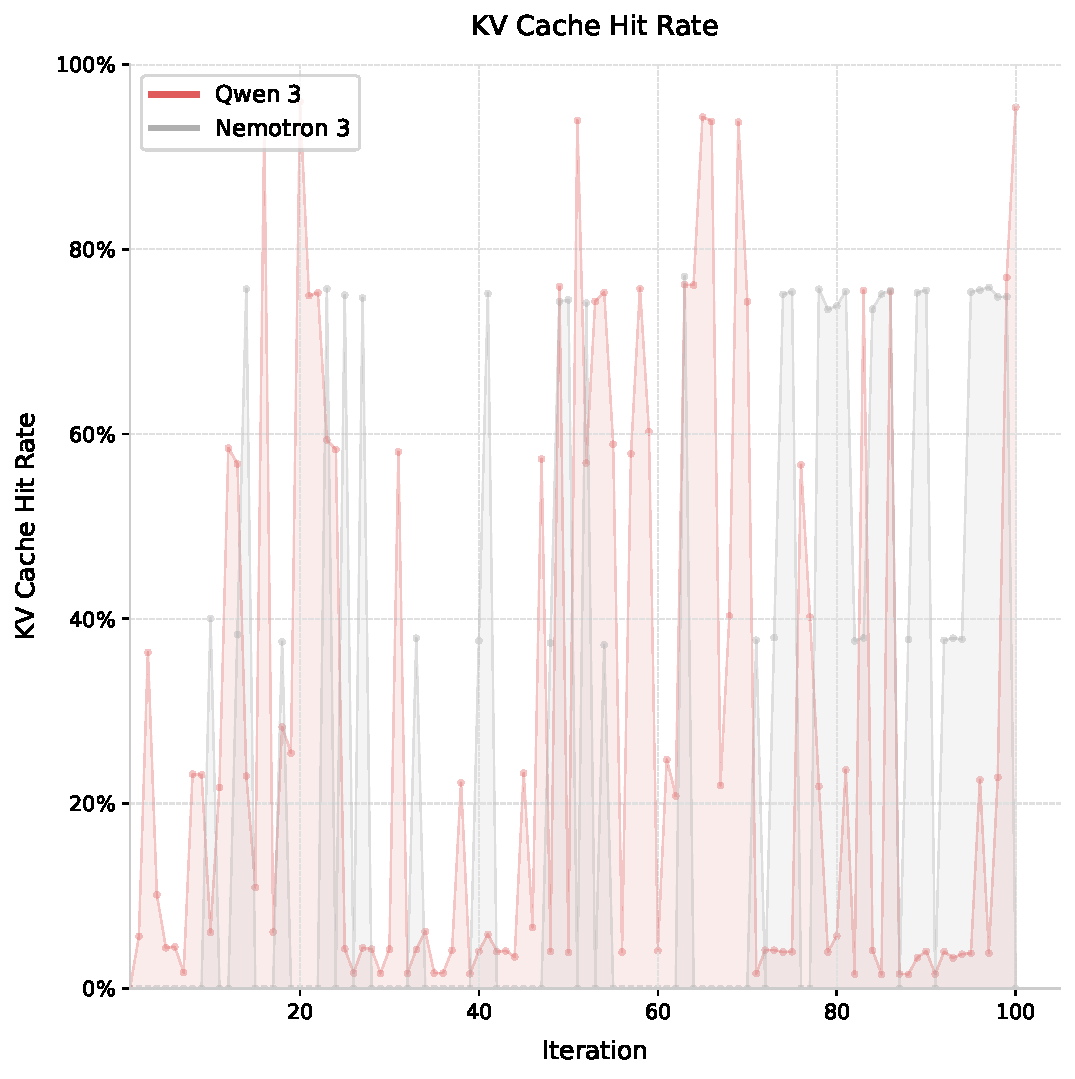
\includegraphics[width=\linewidth]{figures/hit_rate_benchmark.pdf}
\end{minipage}

\caption{
Prompt composition across consecutive AdaEvolve iterations.
Although the overall \textit{content} overlap between prompts can be very high,
most shared content comes from imports, evaluation templates, and task boilerplate
appearing at different positions, resulting in very low \textit{prefix} overlap.
Consequently, vLLM's prefix-based KV cache cannot effectively reuse these tokens.
}
\label{fig:prompt_kv_cache}

\end{figure}
Figure~\ref{fig:prompt_kv_cache} (left) illustrates the prompt composition across consecutive AdaEvolve iterations. In most cases, when two consecutive iterations evolve from different parent programs, the prefix matching chain is already broken inside the \textit{current program} segment. As a result, the only reliably reusable prefix is the static system prompt, which contains only around 200 tokens.

For iterations generated from the same parent program, the current program is identical and the context programs are sampled from the same island, creating a reasonable probability that the first few sampled programs are also identical. In these cases, the total prompt prefix overlap can exceed $30\%$, leading to nontrivial KV cache hit rates. However, this behavior is not guaranteed.

The consistent $0\%$ hit rate is partly caused by the Nemotron hybrid Mamba architecture used during benchmarking, where the KV cache block size is increased to $4224$ tokens to match the SSM state size. As a result, KV reuse only occurs when an entire $4224$-token block matches exactly, so even prompts with moderate prefix overlap can still produce a strict $0\%$ cache hit rate. Standard Transformer models with much smaller cache blocks would generally achieve nonzero hit rates, but reuse would still remain low in most cases since only the shared system prompt is reusable, as illustrated by the Qwen curve in Figure~\ref{fig:prompt_kv_cache} (right). Thus, simply reducing the cache block size does not fundamentally resolve the problem.

This creates an interesting systems challenge: high KV cache reuse prefers highly stable prompts, while evolutionary search algorithms inherently rely on prompt evolution and diversification. Artificially stabilizing the prompt structure may improve cache reuse, but can also reduce search diversity and optimization performance.

Instead of forcing prompts to become more similar, we therefore focus on maximizing the utility of each cached prompt through the following strategies:
\begin{itemize}
    \item Generate multiple child programs from the same cached prompt using batched decoding, amortizing the prefill cost across many candidate generations.
    
    \item Exploit GPU idle time during program evaluation to speculatively pre-generate the next iteration. In this pipeline, the KV cache prefill cost of future generations can be partially overlapped with evaluation latency. While this provides limited benefit in the original AdaEvolve setup with only one child per iteration, the overlap becomes more crucial for the larger evaluation cost of $K$ candidate programs with batching generation.
\end{itemize}


\section{Methods}

We describe the two modifications to \adaev{} that together constitute
EvoScale. Both are implemented entirely in the controller layer and
require no changes to \adaev{}'s underlying database, island machinery,
or evaluator interface.

\subsection{K-Batched Candidate Generation}

In vanilla \adaev{}, each iteration issues a single LLM call built from
one sampled parent program. The key observation is that vLLM's prefix
cache matches blocks by a chained hash of their token content: once the
first call prefills a block, any subsequent call with the same prefix
inherits the cached KV state at zero GPU cost. Vanilla \adaev{} never
exploits this because no two consecutive iterations share the same
prompt.

EvoScale replaces the single call with a fan-out of $K$ calls that all
use the \emph{same} prompt, built once from one parent sample. The
parent is sampled once per iteration, the prompt is constructed once,
and then $K$ asynchronous LLM calls are dispatched concurrently. The
first call to reach vLLM prefills each block and registers it as
\textsc{computing}; the remaining $K-1$ calls wait on that event and
inherit the result with no additional GPU prefill work. To keep the $K$
children diverse despite the shared prompt, we spread temperature
linearly across the $K$ calls around a configured base value. Since
temperature is a decode-time parameter it does not affect the cache key,
so diversity is preserved without changing any block hashes. All $K$
children are added to the island database, but UCB rotation, migration,
and stagnation tracking all advance once per iteration, preserving
\adaev{}'s original schedule.

\subsection{Speculative Iteration Pipelining}

After iteration $t$'s $K$ LLM calls complete but before its evaluations
finish, EvoScale launches a \emph{speculative} fan-out for iteration
$t{+}1$ using a predicted prompt. We use a simple predictor: if the
database's current best program differs from the parent used in
iteration $t$, we build a prompt against it (since \adaev{}'s
exploitation mode tends to pull toward the best-so-far); otherwise we
reuse the current prompt unchanged. When iteration $t{+}1$ actually
starts, the real prompt is compared to the predicted one. On a hit, the
speculative responses are consumed directly and no new LLM call is
needed. On a miss, the speculative tasks are cancelled, but the prefill
they performed still warms the cache for the real call.

Because speculative calls consume vLLM scheduler slots, this policy can
hurt throughput when the GPU is already saturated. We add a pressure
gate: before launching speculation, EvoScale polls
\texttt{vllm:num\_requests\_running} from vLLM's \texttt{/metrics}
endpoint, and skips speculation if the ratio to \texttt{max\_num\_seqs}
exceeds a threshold (we use 0.6). The metrics value is cached
process-wide for 1.5\,s to avoid blocking the event loop on every
iteration.

% -----------------------------------------------------------------------

\section{Experimental Setup}

\subsection{Hardware and Software}

All experiments run on a single node with 8$\times$ NVIDIA H100 80\,GB
GPUs. We use one GPU throughout; the remaining seven are idle. The
inference engine is vLLM 0.15.1 with prefix caching enabled. The model
is \texttt{Qwen/Qwen3-4B-Instruct-2507}, the closest supported Qwen3
variant available in this version of vLLM. The vLLM endpoint is
configured with \texttt{--max-num-seqs 32} and
\texttt{--gpu-memory-utilization 0.85}.

\subsection{Benchmarks}

We evaluate on two mathematical optimization benchmarks from
SkyDiscover's math suite, both using file-based evaluators:

\begin{itemize}
    \item \textbf{\texttt{circle\_packing}}: pack 26 circles in a unit
    square to maximize the sum of radii. The seed solution scores 0.364
    against an AlphaEvolve target of 1.000.
    \item \textbf{\texttt{signal\_processing}}: optimize DSP filter
    coefficients. The seed solution scores 0.499.
\end{itemize}

\subsection{Baselines and Arms}

We compare three configurations:

\begin{itemize}
    \item \textbf{Vanilla}: standard \adaev{} issuing one LLM call per
    iteration ($K{=}1$, no speculation).
    \item \textbf{Batched $K{=}2$, $K{=}4$, $K{=}8$}: EvoScale with the
    respective batch size and no speculative pipelining.
    \item \textbf{Batched + Speculative ($K{=}4,8$)}: EvoScale with $K{=}4,8$
    and GPU-pressure-gated speculative pipelining, prompt matching on
    predicted parent ID.
\end{itemize}

\subsection{Metrics}

We report three primary metrics. \textbf{Cache hit rate} is computed as
$(\textit{cache\_hits} + \textit{shared\_hits}) /
\textit{total\_blocks\_seen}$, where shared hits count blocks inherited
via vLLM's \textsc{computing}-state coordination. \textbf{Per-call wall
time} is the total cohort wall time divided by the number of LLM calls
issued. \textbf{Best score} is the highest \texttt{combined\_score}
achieved by any program in the island database at the end of the run.
All experiments are repeated over multiple seeds and we report mean and
standard deviation across seeds.

\section{Results}

\subsection{Effect of $K$ on Cache Hit Rate}

Table~\ref{fig:hit_rate} shows the KV cache hit rate across both
benchmarks as $K$ increases. At $K{=}1$, hit rates are low (12.6\% and
22.9\% for signal processing and circle packing respectively), reflecting
the fact that each vanilla \adaev{} iteration issues a unique prompt with
no opportunity for intra-iteration cache reuse. Hit rate increases
monotonically with $K$, reaching 84.9\% and 86.3\% at $K{=}8$. This
confirms the core mechanism: all $K$ calls within a batch share an
identical prompt, so only the first call pays the full prefill cost and
the remaining $K-1$ inherit cached KV blocks at zero GPU prefill cost.

% \begin{table}[ht]
% \centering
% \small
% \caption{KV cache hit rate (\%) by benchmark and $K$.}
% \label{tab:hit_rate}
% \begin{tabular}{lcccc}
% \toprule
% Benchmark & $K{=}1$ & $K{=}2$ & $K{=}4$ & $K{=}8$ \\
% \midrule
% Circle Packing    & 22.9 & 65.9 & 76.7 & 84.9 \\
% Signal Processing & 12.6 & 68.5 & 79.1 & 86.3 \\
% \bottomrule
% \end{tabular}
% \end{table}

\begin{figure}[!htbp]
    \centering
    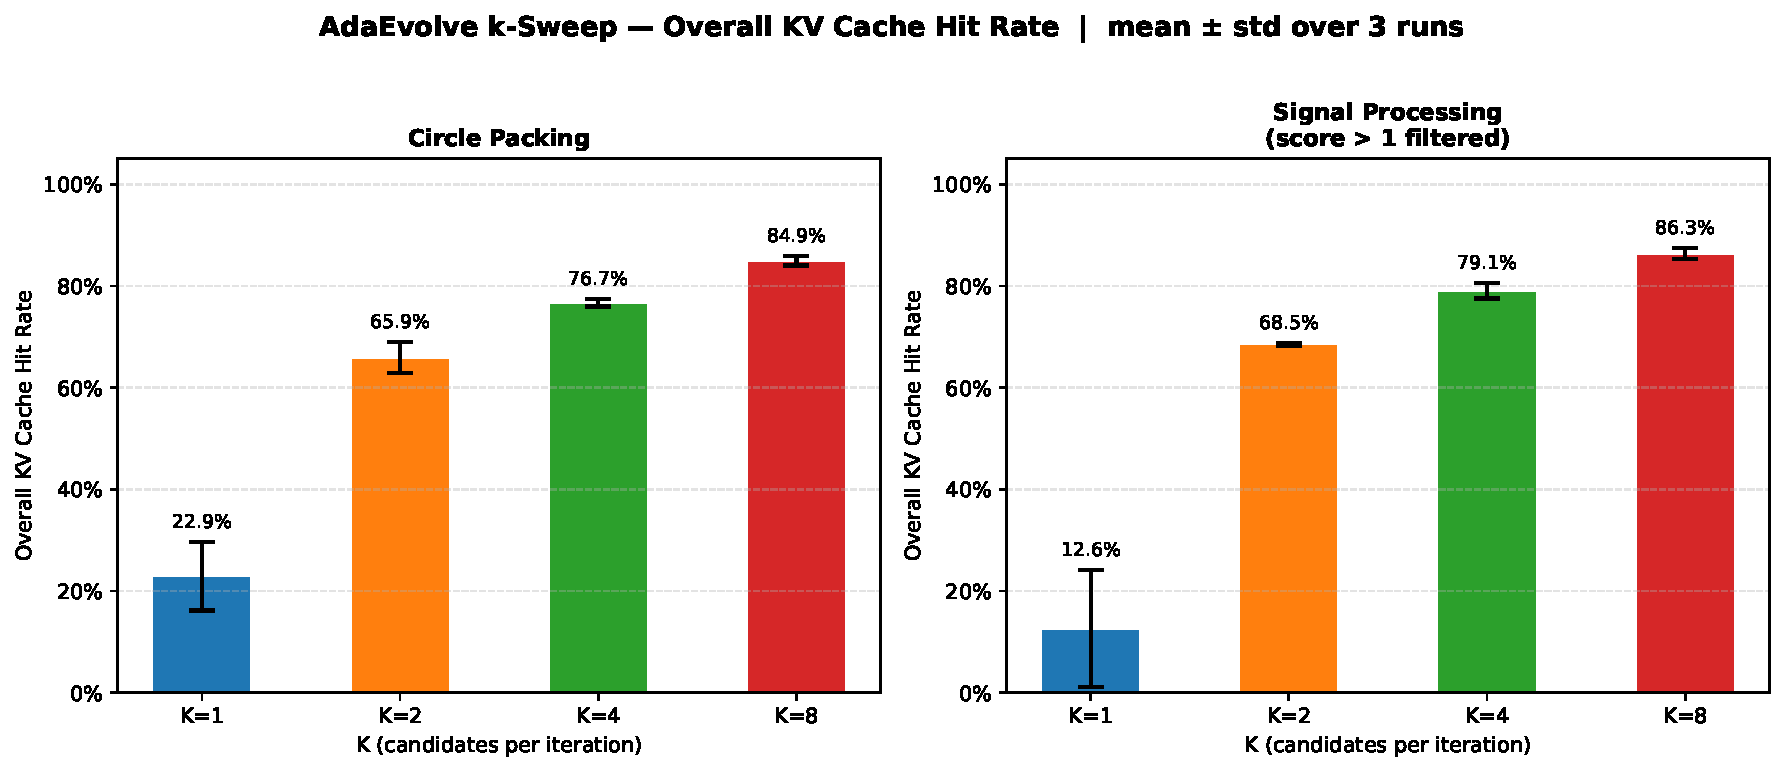
\includegraphics[width=1.0\linewidth]{figures/k_sweep_kv_cache_hit_rate.pdf}
    \caption{
    Overall KV cache hit rate across different batch sizes $K$ for
    Circle Packing and Signal Processing (mean $\pm$ std over 3 runs).
    Both benchmarks exhibit a consistent increase in hit rate as $K$
    grows, with the largest gains occurring between $K{=}1$ and $K{=}2$.
    The trend indicates that larger candidate batches produce substantially
    more reusable prompt prefixes during decoding, leading to more effective
    KV cache reuse across requests.
    }
    \label{fig:hit_rate}
\end{figure}

\subsection{Effect of $K$ on LLM Generation Time per Candidate}

Per-candidate LLM generation time falls substantially as $K$ increases (see the right column of Figure \ref{fig:ksweep}).
For signal processing, per-candidate LLM time drops
from 28.5\,s at $K{=}1$ to 4.6\,s at $K{=}8$, a $6.2\times$ reduction.
Circle packing shows a $4.7\times$ reduction (65.7\,s to 14.0\,s). In
both cases the largest gains occur between $K{=}1$ and $K{=}4$; returns
diminish beyond that, consistent with the cache hit rate beginning to
plateau around 80\% at $K{=}4$ (Table~\ref{tab:hit_rate}).

\subsection{Evaluation Time as a Bottleneck}

The two benchmarks represent qualitatively different bottleneck regimes,
as shown in Table~\ref{tab:eval_time}. Signal processing evaluation is
near-instant (under 1\,s), so LLM time dominates and higher $K$ yields a
large net speedup. Circle packing evaluation is expensive and grows with
$K$: at $K{=}8$, concurrent evaluations contend for resources, pushing
per-candidate eval time to 261.8\,s --- nearly $18\times$ the LLM time at
the same $K$. This means the evaluation bottleneck partially cancels the
LLM savings for circle packing at high $K$, and $K{=}4$ is likely the
practical sweet spot for that benchmark.

\begin{table}[ht]
\centering
\small
\caption{Per-candidate evaluation time (seconds) by benchmark and $K$.}
\label{tab:eval_time}
\begin{tabular}{lcccc}
\toprule
Benchmark & $K{=}1$ & $K{=}2$ & $K{=}4$ & $K{=}8$ \\
\midrule
Circle Packing    & 45.7 & 113.6 & 159.9 & 261.8 \\
Signal Processing &  0.2 &   3.6 &   0.3 &   0.6 \\
\bottomrule
\end{tabular}
\end{table}

\subsection{Search Quality}

Table~\ref{tab:best_score} reports the best score achieved within a
2-hour wall-clock budget (mean $\pm$ std across 3 runs). For circle
packing, scores are high across all $K$ values ($>$0.98) with no strong
trend, suggesting the task is near-saturated within this time budget
regardless of $K$. We also plot the performance in the left column of Figure \ref{fig:ksweep}. Signal processing shows more variance and a modest
improvement from $K{=}1$ to $K{=}4$, but the overall score at $K{=}8$ does not improve
further. Per-candidate improvement rate declines with $K$ on both
benchmarks (circle packing: 9.8\% at $K{=}1$ to 4.3\% at $K{=}8$),
which is expected: siblings within a batch share the same parent and
prompt, so their mutations are correlated and the marginal value of each
additional sibling diminishes. Despite this, the absolute number of
improvements per hour still benefits from higher $K$ because more
candidates are generated per unit time. Furthermore, we observe a quicker saturation in the performance of batching in the signal processing task because the evaluation cost is much lower, and hence runs are much faster. In contrast, batched generation for $K\ge 4$ in the circle-packing task only obtains some advantage in the early stage (15min), but not so much in the long run ($K = 8$ is comparable with $K = 1$).

\begin{table}[ht]
\centering
\small
\caption{Best score at 2 hours (mean $\pm$ std, 3 runs per condition).}
\label{tab:best_score}
\begin{tabular}{lcccc}
\toprule
Benchmark & $K{=}1$ & $K{=}2$ & $K{=}4$ & $K{=}8$ \\
\midrule
Circle Packing    & $0.9947 \pm 0.0016$ & $0.9897 \pm 0.0064$
                  & $0.9957 \pm 0.0020$ & $0.9961 \pm 0.0006$ \\
Signal Processing & $0.5902 \pm 0.0457$ & $0.6540 \pm 0.1077$
                  & $0.6737 \pm 0.0517$ & $0.6678 \pm 0.0645$ \\
\bottomrule
\end{tabular}
\end{table}

\begin{figure}[t]
  \centering
  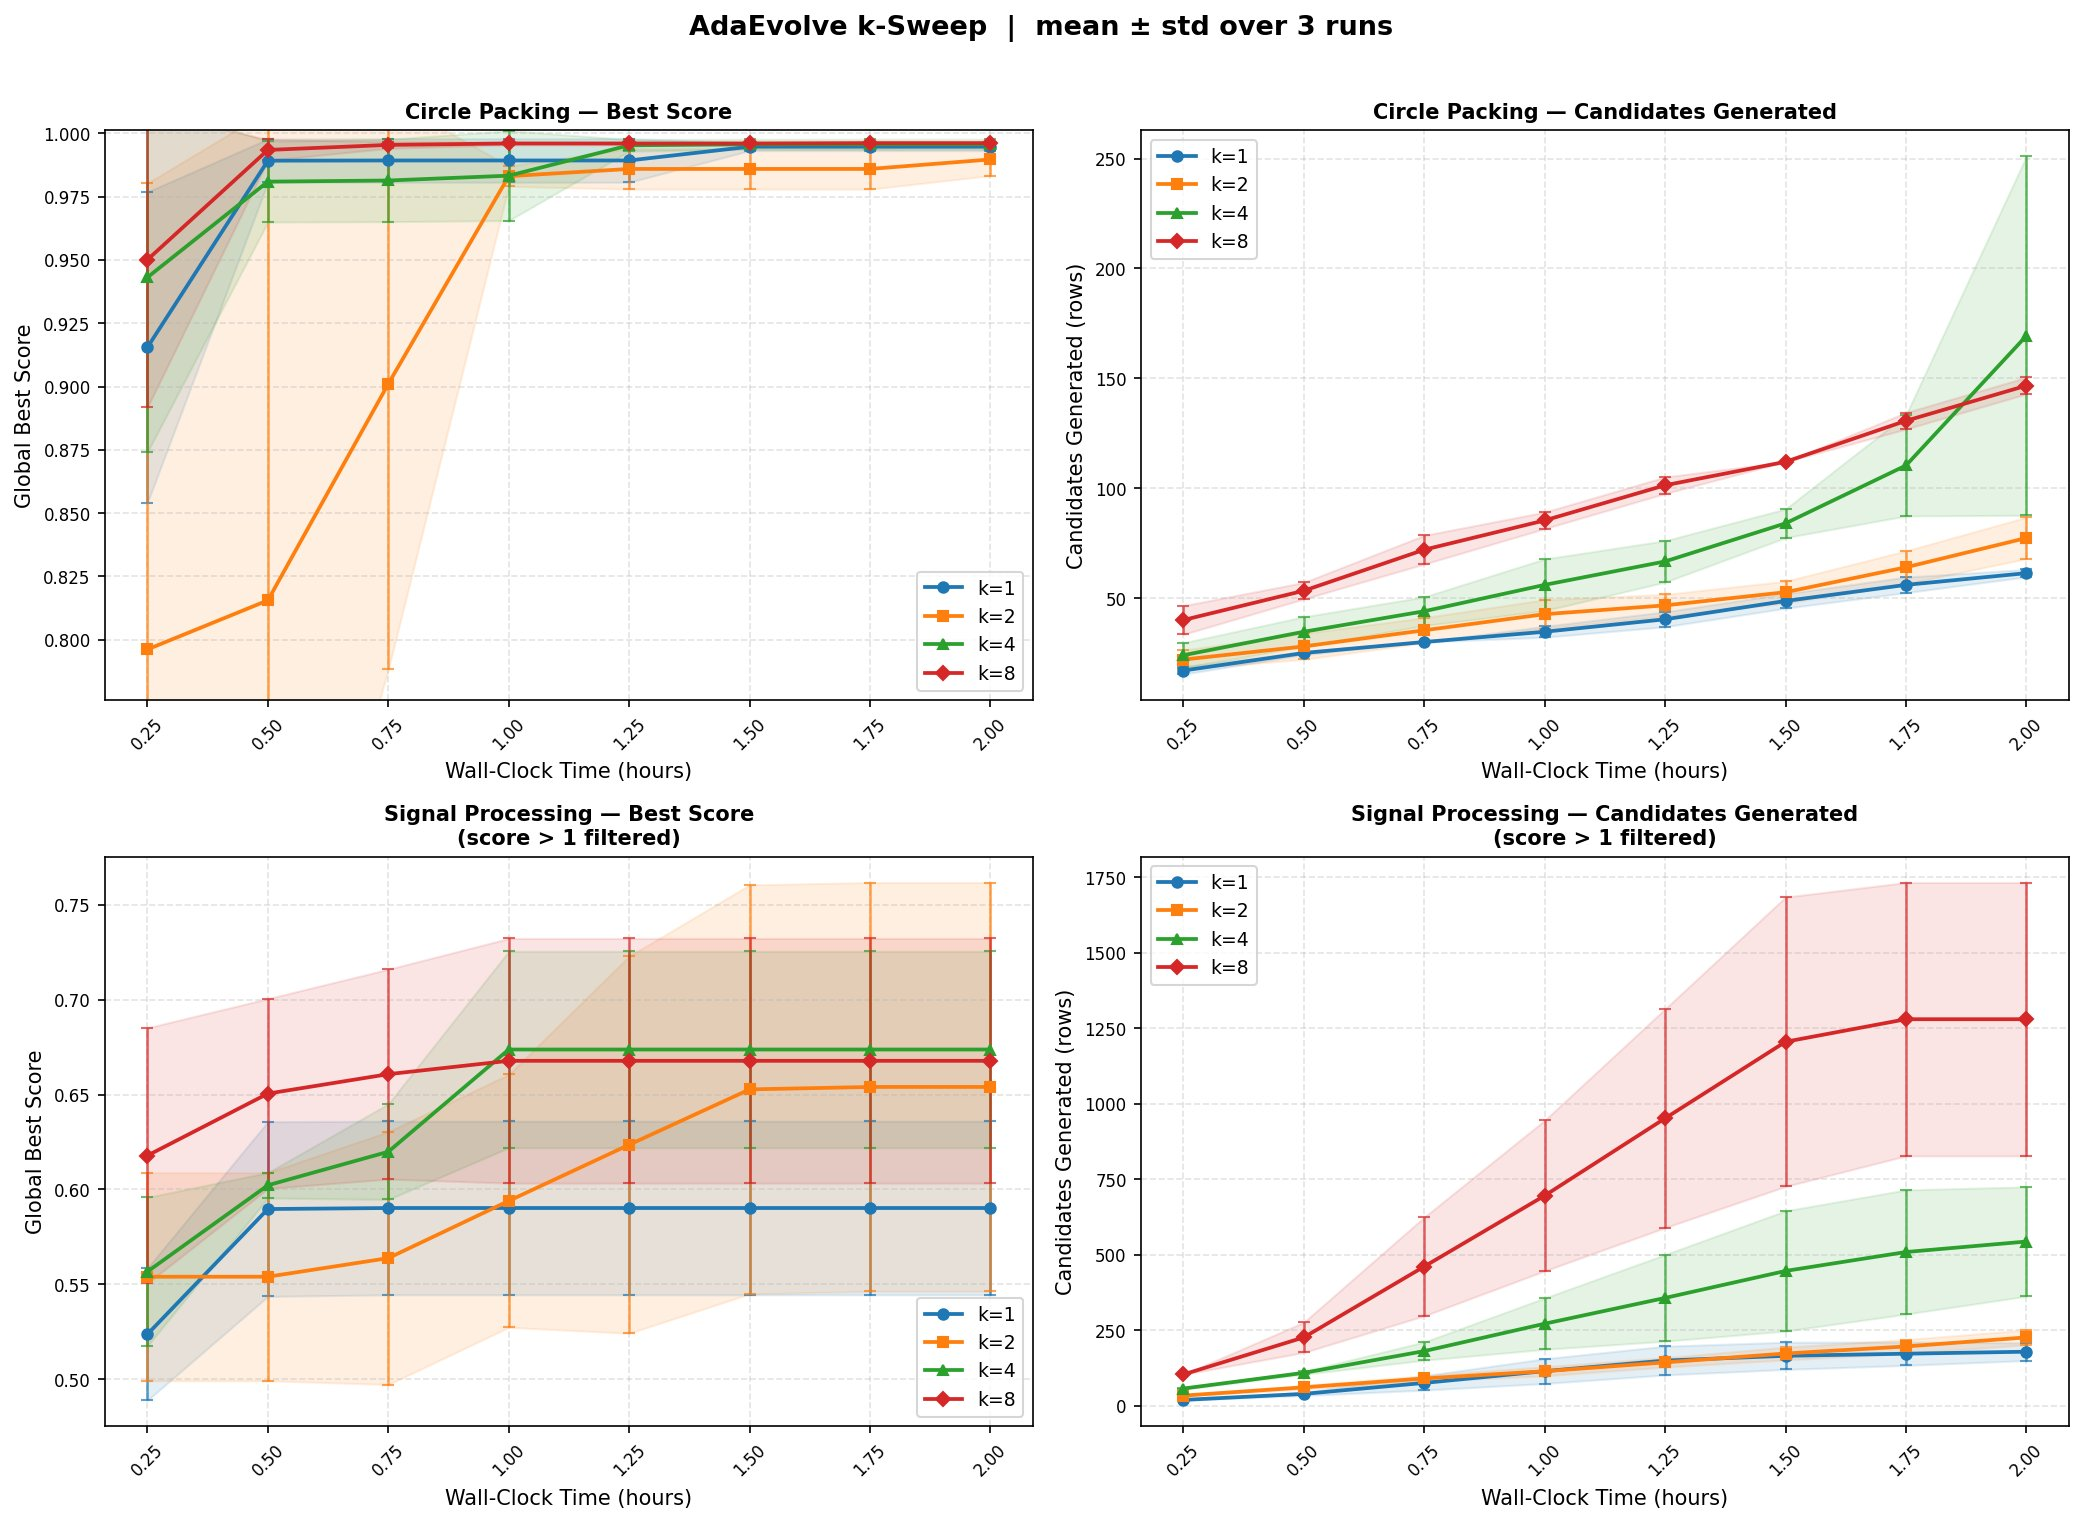
\includegraphics[width=\textwidth]{figures/fig_ksweep.png}
  \caption{\adaev{} $K$ batch candidate sweep: best score (left column) and candidates
  generated (right column) vs.\ wall-clock time for
  $K \in \{1,2,4,8\}$, mean $\pm$ std over 3 runs.
  \textbf{Circle Packing} (top row): all $K$ values saturate near 1.0
  within the 2-hour budget; larger $K$ reaches this plateau faster and
  generates more candidates per hour.
  \textbf{Signal Processing} (bottom row): best score improves
  substantially with $K$, and the candidate throughput gap widens
  dramatically ($K{=}8$ produces $\sim$8$\times$ more candidates than
  $K{=}1$), reflecting the near-zero evaluation cost of this benchmark.}
  \label{fig:ksweep}
\end{figure}

\subsection{Speculative Pipelining}
\label{sec:results-spec}

We evaluate speculative pipelining at both $K{=}4$ and $K{=}8$.
An initial $K{=}8$ smoke run (described in the Methods section) yielded
a 0\% speculation hit rate due to a prompt-comparison bug: the speculative prompt is built before the current
iteration's $K$ children are added to the database, but the actual
next-iteration prompt includes those children in its sibling-history
block. The stored speculative prompt is therefore always stale by $K$
sibling entries relative to the real next-iteration prompt, and the
full string equality check always fails.
The corrected implementation matches on predicted parent ID instead,
which—since approximately 96\% of consecutive batch pairs share the same
parent—yields a high effective hit rate.
The results below reflect this corrected implementation.

\subsubsection{$K{=}4$: Throughput Gains with an Eval-Time Trade-off}

Figures~\ref{fig:k4_best_score} and~\ref{fig:k4_candidates} compare
$K{=}4$ (no speculation) vs.\ $K{=}4$ (spec) on circle packing over
a 2-hour budget.
The speculative variant generates more candidates per unit time
(Figure~\ref{fig:k4_candidates}).
Both configurations converge to $\approx 0.999$ best score by the
end of the run, with speculation achieving a slightly higher score
in the first hour before the non-speculative variant catches up
(Figure~\ref{fig:k4_best_score}).

\begin{figure}[t]
  \centering

  \begin{subfigure}[b]{0.48\linewidth}
    \centering
    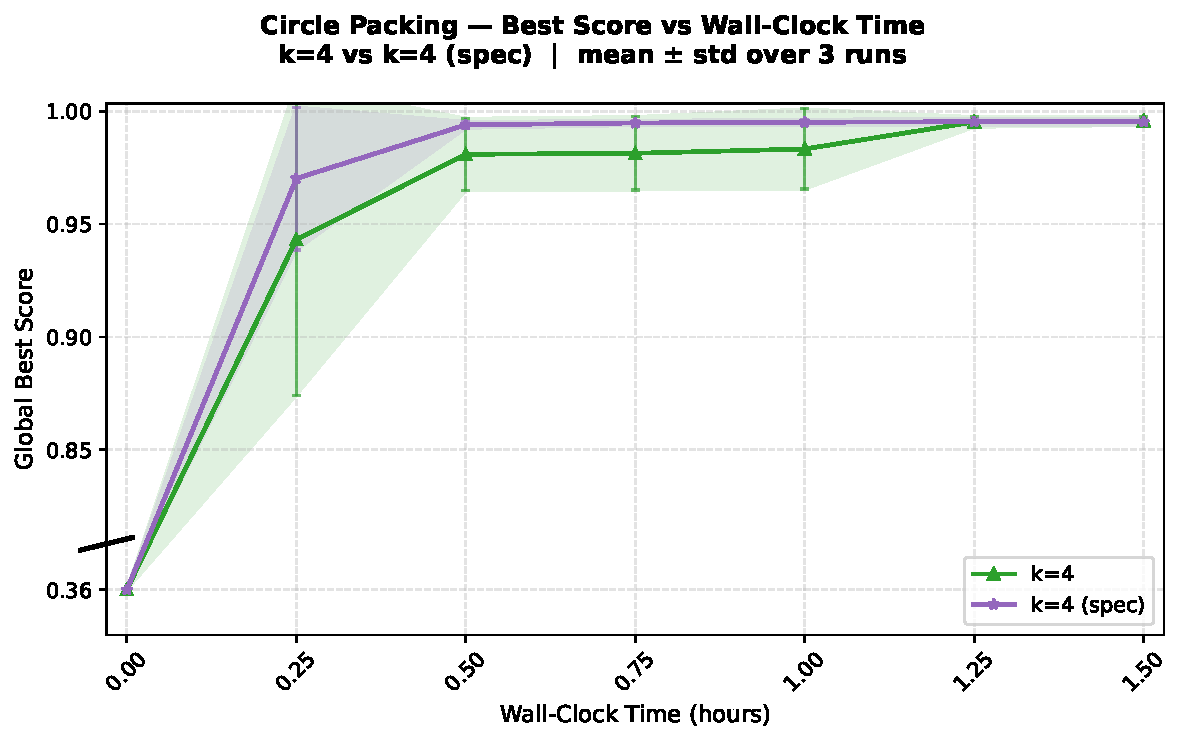
\includegraphics[width=\linewidth]{figures/k4_spec_wallclock_score.pdf}
    \caption{Best score vs.\ wall-clock time.}
    \label{fig:k4_best_score}
  \end{subfigure}
  \hfill
  \begin{subfigure}[b]{0.48\linewidth}
    \centering
    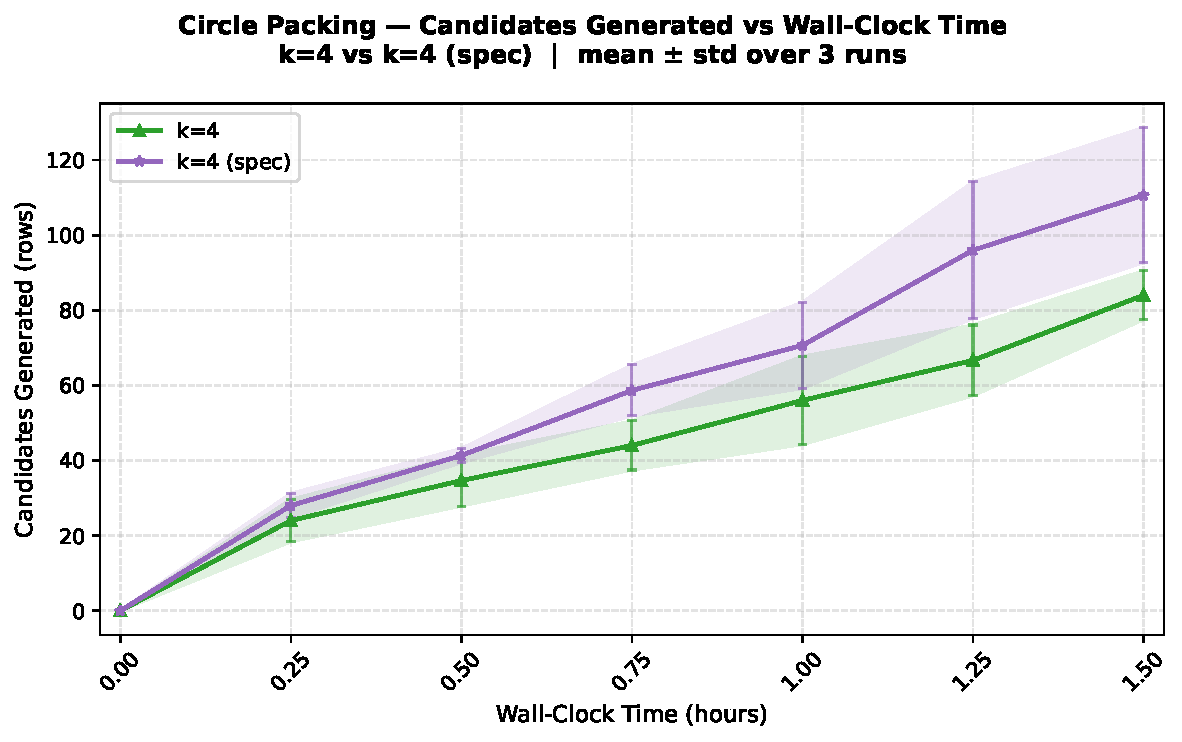
\includegraphics[width=\linewidth]{figures/k4_spec_wallclock_candidates.pdf}
    \caption{Candidates generated vs.\ wall-clock time.}
    \label{fig:k4_candidates}
  \end{subfigure}

  \caption{
  Comparison between standard and speculative generation for
  Circle Packing under $K{=}4$.
  (a) shows the best score over wall-clock time, where speculation
  provides a modest early lead that closes as the task saturates.
  (b) shows the number of generated candidates over time, where
  the speculative variant consistently achieves higher throughput.
  }
  \label{fig:k4_spec_comparison}

\end{figure}

Figure~\ref{fig:k4_spec_breakdown} breaks down mean iteration time
by speculation outcome, pooled across 3 runs
(spec-hit: $n{=}108$; non-hit: $n{=}304$).
Spec-hit iterations have substantially shorter LLM generation time
($49.0\,\text{s}$ vs.\ $95.9\,\text{s}$ mean times) because the speculated call
completes during the previous evaluation window.
However, spec-hit iterations incur \emph{longer} evaluation time
($143.6\,\text{s}$ vs.\ $85.7\,\text{s}$), so net iteration time is
comparable: $192.6\,\text{s}$ (spec-hit) vs.\ $181.5\,\text{s}$
(non-hit).

\begin{figure}[t]
  \centering
  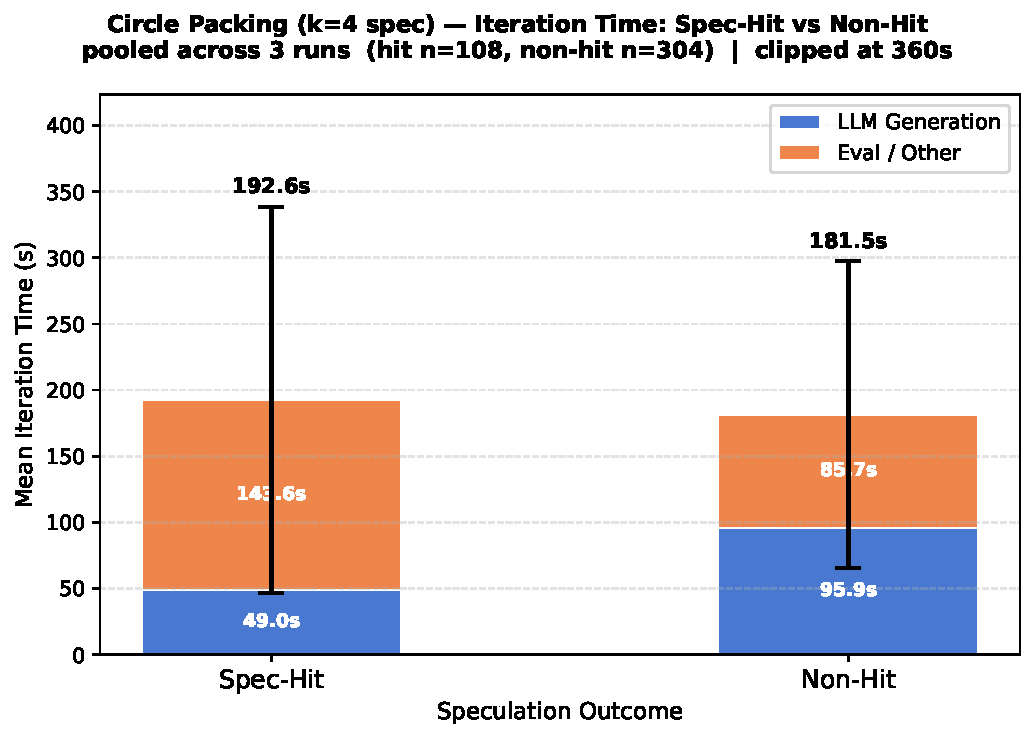
\includegraphics[width=0.62\linewidth]{figures/k4_spec_hit_vs_nohit_time.pdf}
  \caption{Circle Packing ($K{=}4$ spec): mean iteration time
  decomposed into LLM generation and Eval/Other, conditioned on
  speculation outcome. Pooled across 3 runs
  (spec-hit $n{=}108$, non-hit $n{=}304$).
  Spec-hit iterations recover $\sim$47\,s of LLM time but incur
  $\sim$58\,s of additional evaluation latency, leaving total
  iteration wall time roughly even.}
  \label{fig:k4_spec_breakdown}
\end{figure}

The elevated evaluation time on spec-hit iterations is caused by the
speculative predictor's tendency to target the current global-best
program whenever it has changed.
LLM mutations of the global best tend to add extra optimization loops
or increase the iteration count of the candidate program, which
substantially inflates its evaluation runtime.
This bias is a property of the predictor, not of speculation itself,
and could be mitigated by mixing exploitation and exploration targets
in the prediction.
The overall LLM-time effect of speculation across both benchmarks is
quantified in Table~\ref{tab:spec_timing} (§\ref{sec:k8spec}), which
also covers the signal processing benchmark where cheap evaluations
make speculation less beneficial.

\subsubsection{$K{=}8$: System Advantage but Pronounced Quality Regression}
\label{sec:k8spec}

At $K{=}8$, the quality effect is severe while the throughput picture
is mixed.
Figure~\ref{fig:k8_best_score} reveals a pronounced quality regression:
the non-speculative $K{=}8$ run reaches $\approx 0.999$ within 0.5
hours, while $K{=}8$ (spec) stagnates near $0.975$ for the entire
1.75-hour budget.
Despite this, Figure~\ref{fig:k8_candidates} shows that $K{=}8$ (spec)
generates slightly more candidates per unit time throughout the run,
confirming the problem is in search quality, not raw throughput.

\begin{figure}[t]
  \centering

  \begin{subfigure}[b]{0.48\linewidth}
    \centering
    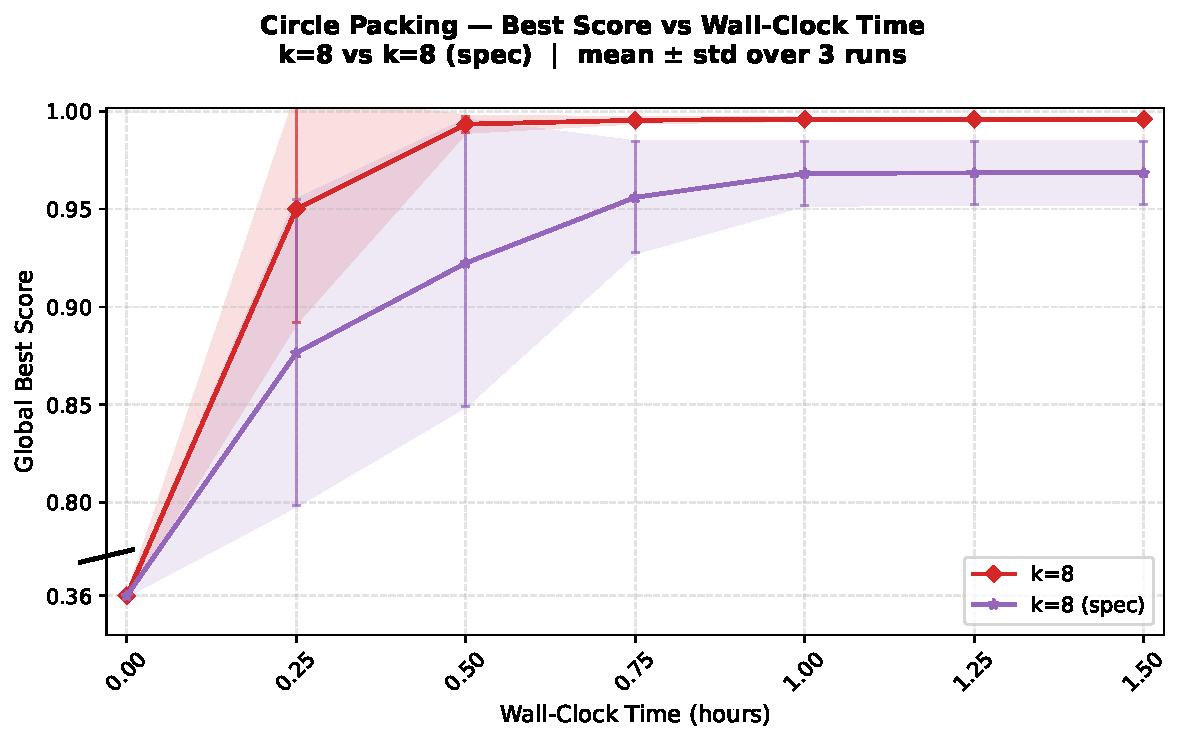
\includegraphics[width=\linewidth]{figures/k8_spec_wallclock_score.pdf}
    \caption{Best score vs.\ wall-clock time.}
    \label{fig:k8_best_score}
  \end{subfigure}
  \hfill
  \begin{subfigure}[b]{0.48\linewidth}
    \centering
    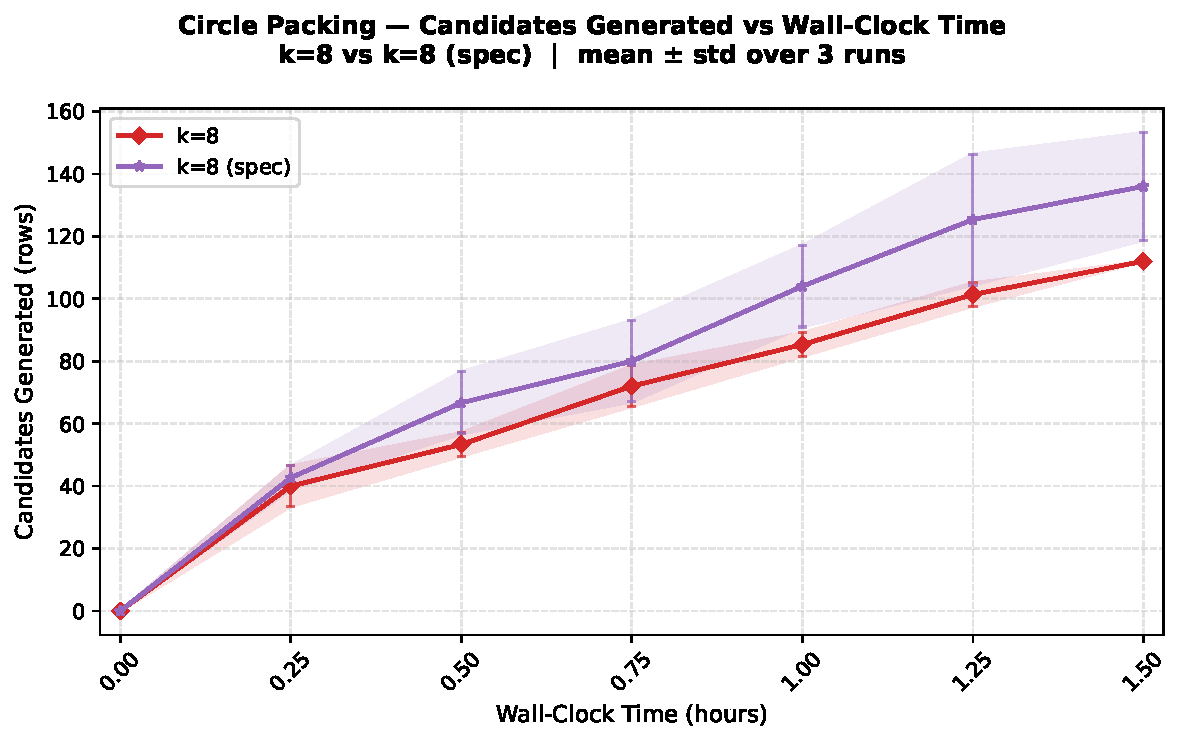
\includegraphics[width=\linewidth]{figures/k8_spec_wallclock_candidates.pdf}
    \caption{Candidates generated vs.\ wall-clock time.}
    \label{fig:k8_candidates}
  \end{subfigure}

  \caption{
  Comparison between standard and speculative generation for
  Circle Packing under $K{=}8$.
  (a) shows a severe quality regression under speculation:
  the non-speculative run saturates near 1.0 within 30 minutes,
  while the speculative variant stagnates around $0.975$.
  (b) shows that the speculative variant still generates slightly
  more candidates per hour, indicating the regression arises from
  degraded search quality rather than insufficient throughput.
  }
  \label{fig:k8_spec_comparison}

\end{figure}
Figure~\ref{fig:k8_spec_breakdown} shows the iteration-time
breakdown for $K{=}8$ spec (spec-hit: $n{=}120$; non-hit: $n{=}424$;
clipped at 360\,s).
Spec-hit iterations achieve shorter LLM time ($44.2\,\text{s}$ vs.\
$99.0\,\text{s}$) \emph{and} shorter eval time ($114.3\,\text{s}$
vs.\ $156.7\,\text{s}$), yielding a total of $158.5\,\text{s}$ vs.\
$255.8\,\text{s}$ for non-hits.
The system efficiency gain is genuine---yet search quality is sharply
degraded.

\begin{figure}[t]
  \centering
  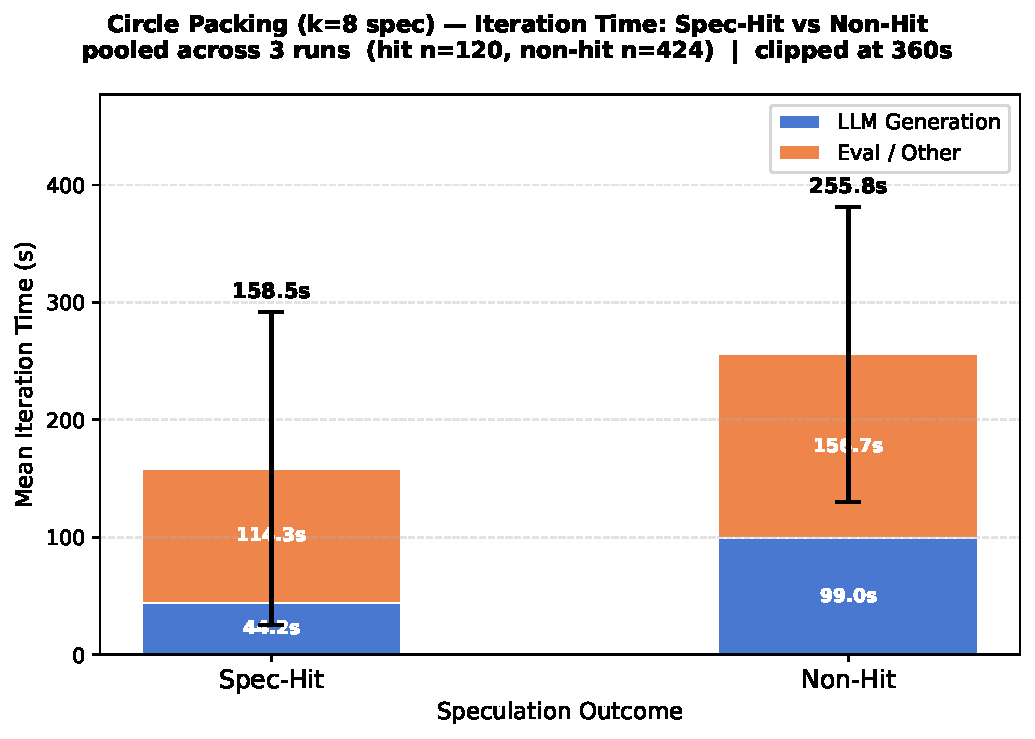
\includegraphics[width=0.62\linewidth]{figures/k8_spec_hit_vs_nohit_time.pdf}
  \caption{Circle Packing ($K{=}8$ spec): mean iteration time by
  speculation outcome, pooled across 3 runs
  (spec-hit $n{=}120$, non-hit $n{=}424$; clipped at 360\,s).
  Spec-hit iterations are faster end-to-end ($158.5$ vs.\
  $255.8\,\text{s}$), yet Figure~\ref{fig:k8_best_score} shows
  this speed comes at a steep search-quality cost.}
  \label{fig:k8_spec_breakdown}
\end{figure}

% Table~\ref{tab:spec_timing} provides a precise breakdown of LLM time
% across speculation conditions for both benchmarks.
% For circle packing, speculation yields a $1.27\times$ LLM-time speedup
% on spec-hit iterations.
% For signal processing---where evaluations are near-instant and
% spec-miss overhead is not amortized by saved eval time---the net effect
% is a $0.87\times$ slowdown, further confirming that speculative
% pipelining is most beneficial when evaluation dominates.

% \begin{table}[ht]
% \centering
% \small
% \caption{Per-iteration timing (mean $\pm$ std, seconds) by speculation
% condition, from the $K{=}8$ speculation runs.
% ``Disabled'' rows show the non-speculative $K{=}8$ baseline.
% LLM speedup is the ratio of Disabled LLM time to Spec-Hit LLM time.}
% \label{tab:spec_timing}
% \begin{tabular}{llrccc}
% \toprule
% \textbf{Benchmark} & \textbf{Condition} & $N$ &
%   \textbf{Iter (s)} & \textbf{LLM (s)} & \textbf{LLM speedup} \\
% \midrule
% \multirow{3}{*}{Circle Packing}
%   & Spec Hit    &  20 & $132.2 \pm 117.9$ & $26.3 \pm 33.1$  & \multirow{3}{*}{\textbf{1.27}$\times$} \\
%   & Spec Miss   &  40 & $159.8 \pm 124.0$ & $63.7 \pm 15.5$  & \\
%   & Disabled    & 512 & $168.0 \pm 181.2$ & $65.3 \pm 47.6$  & \\
% \midrule
% \multirow{3}{*}{Signal Processing}
%   & Spec Hit    &  24 & $56.3 \pm 8.8$    & $51.2 \pm 13.0$  & \multirow{3}{*}{\textbf{0.87}$\times$} \\
%   & Spec Miss   &   8 & $59.8 \pm 12.3$   & $59.6 \pm 12.3$  & \\
%   & Disabled    &1636 & $49.1 \pm 31.8$   & $43.3 \pm 28.8$  & \\
% \bottomrule
% \end{tabular}
% \end{table}

The root cause is a \textbf{prompt-staleness problem amplified by large
$K$}.
When the speculative prompt for iteration $t{+}1$ is constructed,
iteration $t$'s $K$ children have not yet been committed to the island
database.
As a result, the sibling-history block in the speculated prompt is stale
by $K$ entries: none of the $K$ newly generated children are available
as context programs.
At $K{=}4$ this represents 4 missing siblings per speculated iteration;
at $K{=}8$ the staleness is doubled, and consecutive spec-hit
iterations progressively drift from the true island state.
The LLM is therefore guided by a systematically outdated view of the
search population, suppressing the diversity and quality signal that the
multi-island structure is designed to provide.
This effect scales linearly with $K$, explaining why the quality
regression is mild at $K{=}4$ but severe at $K{=}8$.

A clean fix is to delay the speculative prompt construction until the
$K$ children from iteration $t$ have been committed, which preserves
the cache-warming benefit of launching the speculative call early while
ensuring the sibling context is always current.
Alternatively, matching on parent ID rather than prompt content—as
implemented in the corrected version—is a necessary but not sufficient
fix; it resolves the hit-rate accounting bug but does not address the
stale sibling context that causes the quality regression.
We leave a complete resolution to future work.

\section{Limitations}

Several limitations bound the conclusions of this work.

\textbf{Two benchmarks.} All real-hardware results come from
\texttt{circle\_packing} and \texttt{signal\_processing}. These two
tasks happen to represent opposite bottleneck regimes (eval-bound vs.\
LLM-bound), which is useful for understanding the mechanisms, but the
specific numbers---optimal $K$, throughput gains, quality trends---may
not transfer directly to other problem domains.

\textbf{Small run count.} All conditions are averaged over 3 runs.
Standard deviations on best score (Table~\ref{tab:best_score}) are
already non-trivial for signal processing, suggesting that more seeds
would sharpen the quality comparisons.

\textbf{Single model and serving configuration.} Experiments use
\texttt{Qwen3-4B-Instruct-2507} on a single H100 with a fixed vLLM
configuration. Larger models, different block sizes, or multi-GPU
deployments may shift the balance between LLM time and evaluation time,
changing the optimal $K$.

\textbf{Speculative pipelining quality regression.} The stale
sibling-context problem identified in Section~\ref{sec:k8spec} is
unresolved. The parent-ID matching fix corrects the hit-rate accounting
bug but does not eliminate the prompt staleness that causes the quality
degradation at $K{=}8$. Speculative pipelining should therefore be
treated as experimental until a complete fix is implemented.

\textbf{Evaluation contention.} The growth in per-candidate evaluation
time with $K$ for circle packing (45.7\,s at $K{=}1$ to 261.8\,s at
$K{=}8$) is likely caused by resource contention among $K$ concurrent
evaluator processes. We did not isolate the exact cause, so the
practical ceiling on $K$ for eval-heavy benchmarks is not precisely
characterized.

% -----------------------------------------------------------------------

\section{Conclusion}

We presented EvoScale, a cache-aware evolutionary controller that
modifies \adaev{} in two ways: $K$-batched candidate generation, which
fans out $K$ LLM calls per iteration from a shared prompt to exploit
vLLM's prefix cache, and speculative iteration pipelining, which
overlaps LLM generation for the predicted next iteration with the
current iteration's evaluation.

$K$-batched generation is the more reliable of the two contributions.
Across both benchmarks, it raises cache hit rate from 12--23\% at
$K{=}1$ to 85--86\% at $K{=}8$, and reduces per-candidate LLM time by
$4.7$--$6.2\times$. Search quality at a fixed 2-hour budget is
preserved or slightly improved. The main practical caveat is that
evaluation contention grows with $K$ for expensive evaluators, making
$K{=}4$ a safer default than $K{=}8$ for eval-heavy tasks.

Speculative pipelining shows genuine system-level benefit---spec-hit
iterations are faster end-to-end---but introduces a stale sibling
context at large $K$ that suppresses search quality. At $K{=}4$ the
quality effect is mild; at $K{=}8$ it causes a severe regression.
Fixing the prompt staleness (by committing iteration $t$'s children
before constructing the speculative prompt for iteration $t{+}1$) is
the most important next step for this component.

Together, these results suggest that treating the LLM serving stack as
a first-class design concern---rather than a black-box API---opens up
meaningful efficiency gains for evolutionary program search without
requiring changes to the underlying search algorithm.


% -----------------------------------------------------------------------
\newpage
\bibliographystyle{plain}
\begin{thebibliography}{9}

\bibitem{adaevolve2025}
AdaEvolve: Adaptive LLM-Driven Zeroth-Order Optimization.
\textit{arXiv:2602.20133}, 2025.
\url{https://arxiv.org/abs/2602.20133}

\bibitem{deepseekr1}
DeepSeek-AI.
DeepSeek-R1: Incentivizing Reasoning Capability in LLMs via Reinforcement
Learning.
\textit{arXiv:2501.12948}, 2025.

\bibitem{vllm}
W.~Kwon et al.
Efficient Memory Management for Large Language Model Serving with
PagedAttention.
\textit{SOSP}, 2023.

\bibitem{qwen25coder}
Hui et al.
Qwen2.5-Coder Technical Report.
\textit{arXiv:2409.12186}, 2024.

\bibitem{lora}
E.~J.~Hu et al.
LoRA: Low-Rank Adaptation of Large Language Models.
\textit{ICLR}, 2022.
\bibitem{romeraparedes2024funsearch}
B.~Romera-Paredes, M.~Barekatain, A.~Novikov, M.~Balog, M.~P. Kumar,
E.~Dupont, F.~J.~R. Ruiz, J.~S. Ellenberg, P.~Wang, O.~Fawzi, et~al.
\newblock Mathematical discoveries from program search with large language
  models.
\newblock \emph{Nature}, 625:468--475, 2024.

\bibitem{novikov2025alphaevolve}
A.~Novikov, M.~Yasunaga, M.~Balog, et~al.
\newblock {AlphaEvolve}: A coding agent for scientific and algorithmic
  discovery.
\newblock Technical report, Google DeepMind, 2025.
\newblock \url{https://deepmind.google/discover/blog/alphaevolve-a-gemini-powered-coding-agent-for-designing-advanced-algorithms/}

\bibitem{rudes2025openevolve}
R.~Rudes, J.~Hou, and A.~Mehta.
\newblock {OpenEvolve}: Open-source evolutionary program synthesis framework,
  2025.
\newblock \url{https://github.com/ryanrudes/openevolve}

\bibitem{lange2025shinkaevolve}
R.~T. Lange et~al.
\newblock {ShinkaEvolve}: Improving sample efficiency in {LLM}-guided
  evolutionary search.
\newblock Preprint, 2025.

\bibitem{khrulkov2025gigaevo}
V.~Khrulkov, A.~V. Galichin, D.~Bashkirov, D.~Vinichenko, O.~Travkin,
R.~Alferov, A.~Kuznetsov, and I.~Oseledets.
\newblock {GigaEvo}: An open source optimization framework powered by {LLMs}
  and evolution algorithms.
\newblock \emph{arXiv preprint arXiv:2511.17592}, 2025.

\bibitem{cemri2026skydiscover}
M.~Cemri et~al.
\newblock {SkyDiscover}: A unified framework for {AI}-driven scientific
  discovery, 2026.
\newblock \url{https://github.com/skydiscover/skydiscover}

\bibitem{kwon2023pagedattention}
W.~Kwon, Z.~Li, S.~Zhuang, Y.~Sheng, L.~Zheng, C.~H. Yu, J.~E. Gonzalez,
H.~Zhang, and I.~Stoica.
\newblock Efficient memory management for large language model serving with
  {PagedAttention}.
\newblock In \emph{Proceedings of the ACM SIGOPS Symposium on Operating Systems
  Principles (SOSP)}, 2023.

\bibitem{liu2025lmcache}
Y.~Liu, Y.~Cheng, J.~Yao, Y.~An, X.~Chen, S.~Feng, Y.~Huang, S.~Shen,
R.~Zhang, K.~Du, and J.~Jiang.
\newblock {LMCache}: An efficient {KV} cache layer for enterprise-scale {LLM}
  inference.
\newblock \emph{arXiv preprint arXiv:2510.09665}, 2025.

\bibitem{zhong2024distserve}
Y.~Zhong, S.~Liu, J.~Chen, J.~Hu, Y.~Zhu, X.~Liu, X.~Jin, and H.~Zhang.
\newblock {DistServe}: Disaggregating prefill and decoding for
  goodput-optimized large language model serving.
\newblock In \emph{Proceedings of USENIX OSDI}, 2024.

\bibitem{patel2024splitwise}
P.~Patel, E.~Choukse, C.~Zhang, A.~Shah, {\'I}.~Goiri, S.~Maleki, and
R.~Bianchini.
\newblock {Splitwise}: Efficient generative {LLM} inference using phase
  splitting.
\newblock In \emph{Proceedings of the ACM/IEEE International Symposium on
  Computer Architecture (ISCA)}, 2024.

\bibitem{qin2024mooncake}
R.~Qin, Z.~Li, W.~He, M.~Zhang, Y.~Wu, W.~Zheng, X.~Yang, Y.~Zhang,
X.~Wang, K.~Liu, et~al.
\newblock {Mooncake}: Trading more storage for less computation --- a {KV}
  cache-centric architecture for serving {LLM} chatbots.
\newblock \emph{arXiv preprint arXiv:2407.00079}, 2024.

\bibitem{leviathan2023speculativedecoding}
Y.~Leviathan, M.~Kalman, and Y.~Matias.
\newblock Fast inference from transformers via speculative decoding.
\newblock In \emph{Proceedings of the International Conference on Machine
  Learning (ICML)}, 2023.

\bibitem{shao2024deepseekmath}
Z.~Shao, P.~Wang, Q.~Zhu, R.~Xu, J.~Song, X.~Bi, H.~Zhang, M.~Zhang,
Y.~K. Li, Y.~Wu, and D.~Guo.
\newblock {DeepSeekMath}: Pushing the limits of mathematical reasoning in open
  language models.
\newblock \emph{arXiv preprint arXiv:2402.03300}, 2024.

\bibitem{deepseek2025deepseekr1}
{DeepSeek-AI}.
\newblock {DeepSeek-R1}: Incentivizing reasoning capability in {LLMs} via
  reinforcement learning.
\newblock \emph{arXiv preprint arXiv:2501.12948}, 2025.

\end{thebibliography}


\end{document}